\documentclass[10pt,twocolumn,letterpaper]{article}

\usepackage{icb}
\usepackage{times}
\usepackage{epsfig}
\usepackage{epstopdf}
\usepackage{graphicx}
\usepackage{amsmath}
\usepackage{url}
\usepackage{amssymb}
\usepackage[table]{xcolor} % for color coding in correlation Tables

\DeclareMathOperator*{\argmin}{arg\,min}

\newcommand{\superscript}[1]{\ensuremath{^{\textrm{#1}}}}
\def\sharedaffiliation{\end{tabular}\newline\begin{tabular}{c}}

\def\wu{\superscript{*}}
\def\wg{\superscript{\dag}}




% Include other packages here, before hyperref.

% If you comment hyperref and then uncomment it, you should delete
% egpaper.aux before re-running latex.  (Or just hit 'q' on the first latex
% run, let it finish, and you should be clear).
%\usepackage[pagebackref=true,breaklinks=true,letterpaper=true,colorlinks,bookmarks=false]{hyperref}

%\icbfinalcopy % *** Uncomment this line for the final submission

\def\icbPaperID{****} % *** Enter the IJCB Paper ID here
\def\httilde{\mbox{\tt\raisebox{-.5ex}{\symbol{126}}}}


% Pages are numbered in submission mode, and unnumbered in camera-ready
\ificbfinal\pagestyle{empty}\fi
\begin{document}

%%%%%%%%% TITLE
\title{Recompression effects in iris segmentation}

\author{Thomas Bergmueller\wg\wu, Elefterious Christopoulos\wu, Martin Schnoell\wu and Andreas Uhl\wu \\
\wu University of Salzburg, Austria \\
\wg Authentic Vision, Austria\\
{\tt\small tb@authenticvision.com, \{echristop, mschnoell, uhl\}\@cosy.sbg.ac.at}
}





\maketitle
\thispagestyle{empty}

%%%%%%%%% ABSTRACT
\begin{abstract}
	%Iris biometrics data is nowadays usually stored in raw image form. In large scale data bases, e.g. the Aadhaar project, the need for lossy compression emerges to achieve efficient storage. Operating with compressed data impacts 	on the overall performance of an iris recognition system, especially on iris segmentation.
	
	Rating a compression algorithm's
	performance is usually done in experimental studies, where researchers have frequently used JPEG pre-compressed data. It is not clear yet,
	whether results of such compression experiments are reliable if conducted from pre-compressed data. 
	To investigate this issue, we study the impact of using pre-compressed data on iris segmentation and evaluate the relation between iris segmentation 
	performance and general quality metrics. Furthermore we propose a method to overcome potential problems in case using
	pre-compressed data sets cannot be avoided, e.g. for reasons of ground-truth availability.
\end{abstract}

%%%%%%%%% BODY TEXT
\section{Introduction}

Iris recognition \cite{BBurge13a,Rathgeb12e} is one of the most deployed biometric
modalities, standardized by the International Civil Aviation
Organization (ICAO) for use in future passports, and one of
the technologies in the Unique Identification Authority of
India's (UID) Aadhaar project to uniquely identify Indian
citicens. The increasing market saturation of
biometric instead of conventional access control methods
raises the need for efficient means to store such data. The
International Organization for Standardization (ISO)
specifies iris biometric data to be recorded and stored in (raw)
image form (ISO/IEC FDIS 19794-6) rather than in extracted
templates (e.g. iris-codes). Such
deployments benefit from future improvements (e.g. in
feature extraction stage) which can be easily incorporated
without re-enrollment of registered users. Since biometric templates may depend on patent-registered
algorithms, databases of raw images also enable more
interoperability and vendor neutrality \cite{Rathgeb12e}. These facts
motivate detailed investigations and optimisations of image
compression on iris biometrics in order to provide an efficient
storage and rapid transmission of raw biometric records.
Furthermore, the application of low-powered mobile sensors
for image acquisition, e.g. mobile phones, raises the need for
reducing the amount of transmitted data.

%The certainly most relevant standard for compressing image data relevant in biometric systems is the ISO/IEC 19794 standard on Biometric Data Interchange Formats, where in the most recently published version (ISO/IEC FDIS 19794-6), only JPEG2000 is included for lossy compression. JPEG2000 has also been recommended for various application scenarios and standardised iris images (IREX records) by the NIST Iris Exchange\footnote{IREX \url{http://iris.nist.gov/irex/}} program. The ANSI/NIST-ITL 1-2011 standard on ``Data Format for the Interchange of Fingerprint, Facial \& Other Biometric Information'' (former ANSI/NIST-ITL 1-2007) also supports only JPEG2000 for applications tolerating lossy compression.

As a consequence, according to the importance of this issue, many studies comparing and optimising lossy compression techniques for iris imagery 
may be found in the literature. Since the CASIA iris datasets have been very popular among researchers ever since their establishment,
many papers dealing with compression have been relying on the (extended) CASIA V1.0 dataset, including also first IREX investigations 
\cite{BRakshit07a,BIves08a,Matschitsch07a,Haemmerle09a,Konrad09a} (apart from other examples using the ICE 2005 dataset 
% noch V1: BIves05a,Konrad09b,Kostmajer09a,BRakshit06a,
\cite{BDaugman08a,BIves10a}).
	
Since it has been pointed out \cite{BPhilips07a} that the CASIA V1.0 dataset exhibits manipulated pupil areas and should therefore not be used any further in experimentation, compression researchers moved to other (and more recent, more challenging etc.) datasets, e.g. 
	the CASIA V3.0 \cite{Horvath11b,Rathgeb12e}, 
	the CASIA V4.0 \cite{BTuba12a}, the Bath \cite{BIves08a,BPardamean12a}, and the UBIRIS.v1 \cite{Haemmerle09a,BCarneiro11a} datasets.
	While the images of CASIA V1.0 and ICE 2005 are given in uncompressed format, images in CASIA V3.0, CASIA V4.0, UBIRIS and Bath datasets are provided as JPEG (the first three) or JPEG2000 (the latter) lossy compressed data. Therefore, any compression experiments conducted on these datasets operate on pre-compressed data. 
	
	This fact has not been ignored entirely -- for example, in \cite{Rathgeb12e}, preparatory JPEG compression experiments with uncompressed data reveal that 
	slightly pre-compressed data leads to better recognition performance due to denoising effects. Thus experiments with pre-compressed data are assessed to
	be unproblematic. The same argument is used for JPEG2000 pre-compressed data \cite{BPardamean12a} based on the results in \cite{BIves08a}.
	However, eventual artifacts resulting from recompression effects are not accounted for in these considerations. Recompression artifacts arise in cases where	data is compressed twice (or multiple times) with lossy compression schemes, i.e. where artifacts from the first compression step (termed pre-compression)
	are aggravated or exploited by the second compression step.
	
	Two different types of such effects may be distinguished: First, \emph{intra-recompression}, where the same compression scheme is used several times, whereas
	in \emph{inter-recompression} different methods are used in the different compression steps. For example, using JPEG pre-compressed data and applying
	JPEG XR and JPEG2000 \cite{Horvath11b} or JPEG2000 and fractal compression \cite{BCarneiro11a} is eventually prone to inter-recompression
	artifacts, while the application of JPEG to JPEG pre-compressed data \cite{BTuba12a,Rathgeb12e} can be prone to intra-recompression artifacts.
	
	While next to nothing can be found on the issue of inter-recompression artifacts in the general compression literature, 
	intra-recompression artifacts are better investigated, at least in the case of lossy JPEG compression. Soon after the establishment of
	the JPEG standard \cite{Pennebaker93a}, it was found that JPEG recompression artifacts arise and do not follow a linear behaviour \cite{Chan92a}.
	Extensive experiments in this direction can also  be found in \cite{Kumar11a}, and following these obversations, requantisation-based schemes have been
	suggested for JPEG, reducing recompression artifacts considerably \cite{Bauschke03a}. Recently, the identification of images which underwent 
	JPEG double compression (i.e. JPEG intra-recompression) has been a hot topic in image forensics \cite{Sencar12a}.
	
	Taking all these facts together, it gets clear that recompression artifacts may impact experimental results with respect to biometric recognition
	performance, an issue, that has been neglected so far. As discussed, ISO/IEC FDIS 19794-6 requires storing biometric data as raw images, hence all components of a biometric system are affected when operating with compressed data. As we investigate the recompression issue by studying impact on an iris recognition system, the influence on segmentation and texture extraction as well as feature extraction, i.e. iris code computation, has to be evaluated. \cite{severeCompression, BDaugman08a} suggest that data reduction has the highest impact on the iris segmentation. Since segmentation is also the first step in the pipeline, this potentially effects the performance of later steps as well and is therefore of particular importance. 
	
We systematically investigate eventual intra- and inter-recompression effects in an experimental study for iris segmentation. Given the importance of JPEG (as the CASIA V3.0/V4.0 and UBIRIS.v1 datasets are only available in this format), we focus on JPEG pre-compressed data. In our experiments, we compare iris segmentation and general purpose image quality metrics applied	to single compressed vs. recompressed (i.e. JPEG pre-compressed) iris image data. Section \ref{section:comprScheme} discusses relevant aspects on generating single- and recompressed data. The used data sets and methods are described in section \ref{section:exSetup}. Section \ref{section:eval} introduces several experiments and lists their results, which are then compared in section \ref{section:comparison}. From the experiments' individual and comparison results, we draw conclusions in section \ref{section:conclusion}.
	

\section{Compression scheme}
\label{section:comprScheme}
As discussed, we investigate whether there is a difference in using truly uncompressed data or pre-compressed data in experiments rating the performance of an iris segmentation. 
Using pre-compressed data means a pre-compressed image $I_p$ is compressed a second time, resulting in an recompressed image $I_r$. When compressing a truly uncompressed image $I_u$, the resulting image $I_s$ is generated in a single compression step. Since experiments are typically carried out on a data set with more than one image, we denote $I_u^{(k)}, I_p^{(k)}, I_s^{(k)}, I_r^{(k)} \in \mathbb{R}^{w \times h}$ as the $k^{th}$ image with width $w$ and height $h$. For simplicity, $I_u, I_p, I_r, I_s$ subsequently denote a particular image but unspecified image of a data set. Furthermore, we define $s(F) \in \mathbb{N}$ with $F \sim{I \in \mathbb{R}^{w \times h}}$ as a function that returns the file size of the file $F$ storing an image $I$. Since common lossy compression algorithms also employ lossless compression methods, e.g. run-length encoding, before writing to a file, $F$ is only loosely related to the pixel data, namely the image, $I$. For simplicity, we denote $s(I)$ as the file size of the file $F$ encoding the pixel values of an image $I$. $c_{m}(I, q)$ with $q \in \mathbb{N}$ describes the process of compressing an image $I$ using a particular method $m$ parametrized with the quality parameter $p$. In terms of this paper we use the values $m \in \{jpg, jxr, j2k\}$, where 
\begin{itemize}
	\item $jpg$ corresponds to the well-known (ISO/IEC IS 10918-1) DCT-based image compression method JPEG, % \cite{jpg},
	\item $j2k$ corresponds to the wavelet-based image compression standard JPEG2000 (ISO/IEC IS 15444-1), which can operate at higher compression ratios %\cite{j2k}
	and
	\item $jxr$ corresponds to a compression standard JPEG-XR based on Microsoft’s HD Photo, which is specified in (ISO/IEC IS 29199-2). % \cite{jxr}.  
\end{itemize}

For rating an image $I$'s compression effectiveness, we define the compression ratio $cr$ between an uncompressed image $I_u$ and a compressed image $I_c$ as 
\begin{equation}
cr(I_u, I_c) = \frac{s(I_u)}{s(I_c)} \quad \text{with} \quad I_c \in \{I_r, I_s\}
\end{equation}

For the later described experiments, images are compressed to a target compression ratio $cr_t \in \mathbb{R}$. However, only the \emph{j2k} compression standard allows to specify a target compression ratio $cr_t$ directly via parameter $q$. Hence this is the only method where we can control the file size $s(I_c)$ directly. The other two compression methods take a quality parameter $q \in \mathbb{N}$ only, controlling the quality but not the file size $s(I_c)$. Thus it is not possible to set this parameter to meet a certain target compression ratio $cr_t$. Due to the quality parameter's limited universe, the target compression ratio $cr_t$ cannot be achieved exactly for any of the three methods. Parameter optimisation can be done, such that $cr_t \approxeq cr(I_u^{(k)}, I_c^{(k)})$. We propose an algorithm to compress a set of $K$ uncompressed images $I_u$ using a particular method $m$ to achieve a certain compression ratio $cr_t$ in a way that the compression ratio of each image is met as close as possible. 
This process, illustrated in Fig. \ref{fig:comprScheme}, employs
\begin{enumerate}
	\item Compute the single-compressed image $I_s^{(k)}$ with method $m$ such that $cr(I_u^{(k)}, I_s^{(k)}) \approx cr_t$. The optimal quality parameter $q_s^{(k)}$ is computed for each image separately by
	\vspace{-5mm}
	\begin{eqnarray}
	s_t^{(k)} = \frac{s(I_u^{(k)})}{cr_t} \\
	q_s^{(k)} = \underset{q \in \mathbb{N}}{argmin}|s(c_m(I_u^{(k)},q)) - s_t^{(k)}|,
	\end{eqnarray} where $s_t^{(k)}$ is the file size exactly meeting the target compression ratio $cr_t$. This is implemented by iteratively searching the quality parameter $q$ that results in the closest achievable compression ratio $cr(I_u, I_c)$. The single compressed images $I_s^{(k)}$ using method $m$ are computed with the optimal parameters $ q_s^{(k)}$ as
	\begin{equation}
	I_s^{(k)} = c_m(I_u^{(k)}, q_s^{(k)})
	\end{equation}
	
	\item Compute a pre-compressed image $I_p^{(k)}$ using $jpg$-method with an arbitrary but fixed quality parameter $q_p$, i.e. 
	\begin{equation}
		I_p^{(k)} = c_{jpg}(I_u^{(k)}, q_p)
	\end{equation}
	
	\item Now, find a quality parameter $q_d^{(k)}$ that allows to compress the pre-compressed image $I_p^{(k)}$ a second time, such that the resulting recompressed image $I_r^{(k)}$ has the same file size as the single-compressed image $I_s^{(k)}$, i.e. $s(I_s^{(k)}) \approxeq s(I_r^{(k)})$. Such a quality parameter $q_r^{(k)}$ can be found by optimising
	\begin{eqnarray}	
		q_r^{(k)} = \underset{q \in \mathbb{N}}{argmin}|s(c_m(I_p^{(k)},q)) - s(I_s^{(k)})| \\
		\forall s(I_s^{(k)}) \geq s(I_r^{(k)})
		\label{equ:recomp}
	\end{eqnarray}
	\vspace{-5mm}
	
The condition $s(I_s^{(k)}) \geq s(I_r^{(k)})$ is of importance to establish fair conditions, since it is very likely that the file sizes $s(I_s^{(k)}), s(I_r^{(k)})$  cannot be equalized due to the limited universe of the quality parameters $q$. The recompressed images $I_r^{(k)}$ are then computed from the pre-compressed images $I_p^{(k)}$ with the found optimal parameters $q_r$ as
	\vspace{-2mm}
	\begin{equation}
	I_r^{(k)} = c_m(I_p^{(k)}, q_r^{(k)})
	\end{equation}
\end{enumerate}


\begin{figure}
	\begin{center}		
		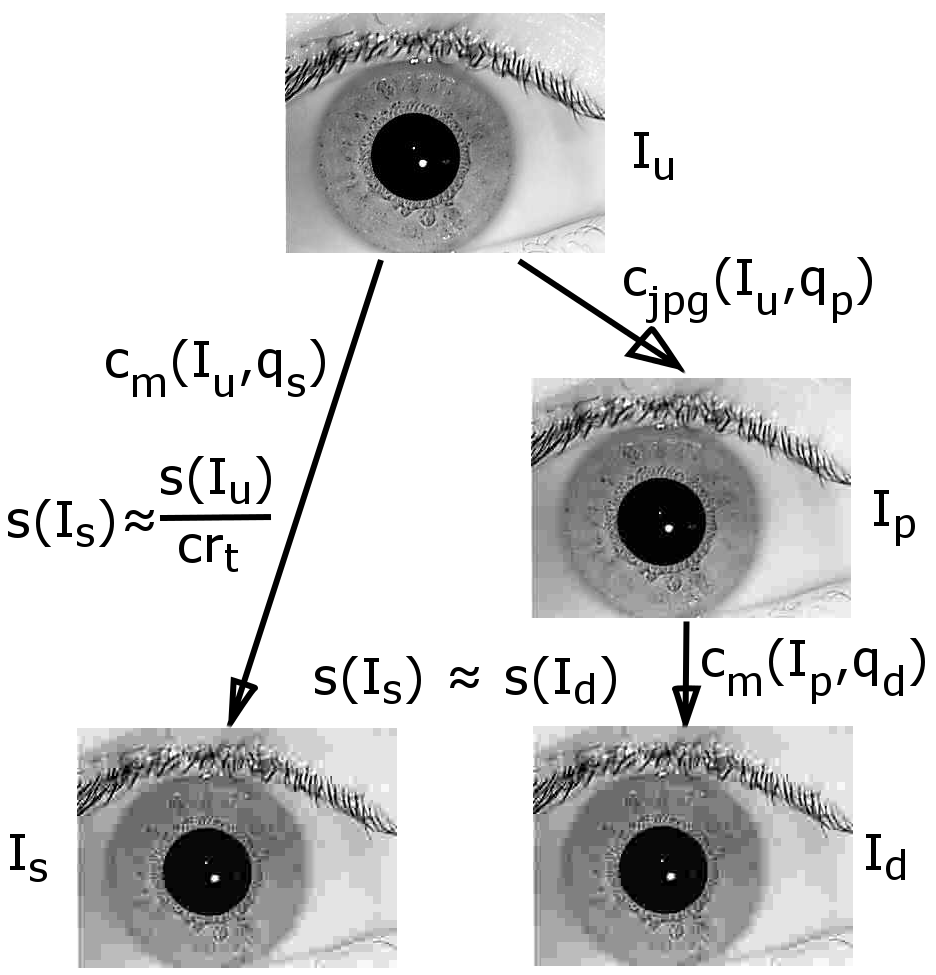
\includegraphics[width=0.5\linewidth]{img/comprScheme}
	\end{center}
	\caption{Compression principle to obtain two images achieving approximately the same target compression ratio $cr_t$ from an uncompressed image $I_u^{(k)}$ using a particular compression method $m$. One image, $I_s^{(k)}$, is compressed in a single step while the other, $I_r^{(k)}$, uses a pre-compression and a final compression step. The pre-compression step is always a $jpg$-compression, while the final one uses the same method $m$ as used in single-compression.}
	\label{fig:comprScheme}
	
\end{figure}


Using data sets generated with this method, we can investigate the impact of artifacts in an recompressed image $I_r$ in comparison to those in single-images $I_s$. The first one contains artifacts by two compression, while the latter one contains artifacts from one compression step only.

\section{Experimental setup}
\label{section:exSetup}
Although there are several iris data sets around, few are available in uncompressed format. We use the IITD Iris data base\footnote{IITD Iris Database version 1.0, www4.comp.polyu.edu.hk/\textasciitilde csajaykr/IITD/Database\_Iris.htm}. The main reason for this is the availability of a segmentation ground truth created by an expert, which was recently introduced by Hofbauer \etal \cite{Hofbauer14b} and used in \cite{severeCompression}. The $k^{th}$ image of this segmentation ground truth data set is subsequently denoted as $SGT^{(k)}$. 
According to information by the IITD iris data base's authors, the images, stored in a 3-channel uncompressed bitmap format\footnote{We want to point out that storing in 1-channel bitmaps would be more efficient, since the images were captured in near-infrared. However, we use the size information of the 3-channel bitmap in computing compression ratios} are already JPEG-compressed with 100\% quality by the sensor (JIRIS, JPC1000). Since they are stored as bitmaps, all images have an identical file size of $s(I_u)$=230,454 bytes. Despite not being optimal, using the IITD was necessary due to the available ground truth, for reasons becoming obvious in section \ref{section:ser}. Futhermore, the IITD -- contrary to others, e.g. the ND-IRIS-0405 iris image dataset \cite{Bowyer_thend-iris-0405} -- is captured under favorable conditions, which allows for lower segmentation errors. This is necessary to distinguish between noise and recompression-effects. We use the scheme introduced in section \ref{section:comprScheme} to compress obtain data sets with target compression ratios $cr_t \in \{15, 20, 25, ..., 70, 75\}$. For each of these target compression ratios $cr_t$, the pre-compression step in recompression mode is carried out with quality parameters $q_p \in \{100, 80, 75, 70\}$ to simulate different levels of pre-compression. Each of these combinations is used to compress with the introduced $jpg$, $j2k$ and $jxr$ methods. We start at compression ratio $cr_t=15$, because even a pre-compression with $q_p=100$ achieves - depending on the image's content - already a compression ratio of $cr(I_u, I_p) \approx 10$. For obvious reasons, no smaller compression ratio $cr(I_u, I_r) < cr(I_u, I_p)$ can be reached in recompression. This results in a total of 195 data sets with 2240 images each, whose distribution is shown and discussed in fig. \ref{fig:dataDistribution}.

\begin{figure}
	\begin{small}
	
	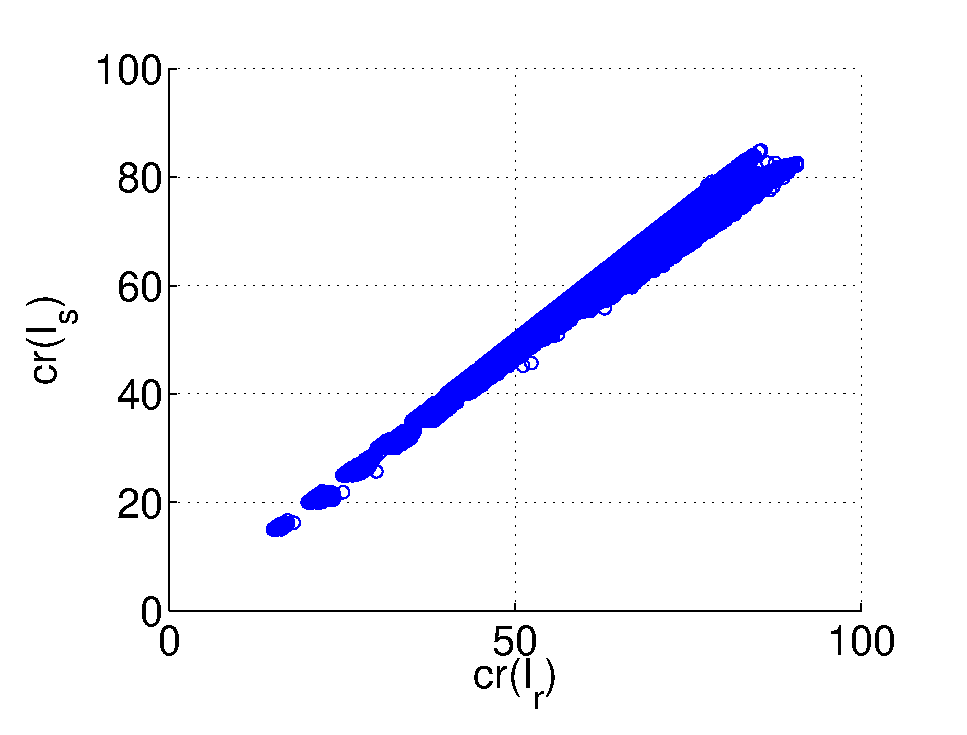
\includegraphics[width=0.45\linewidth]{img/jpgData.eps}
	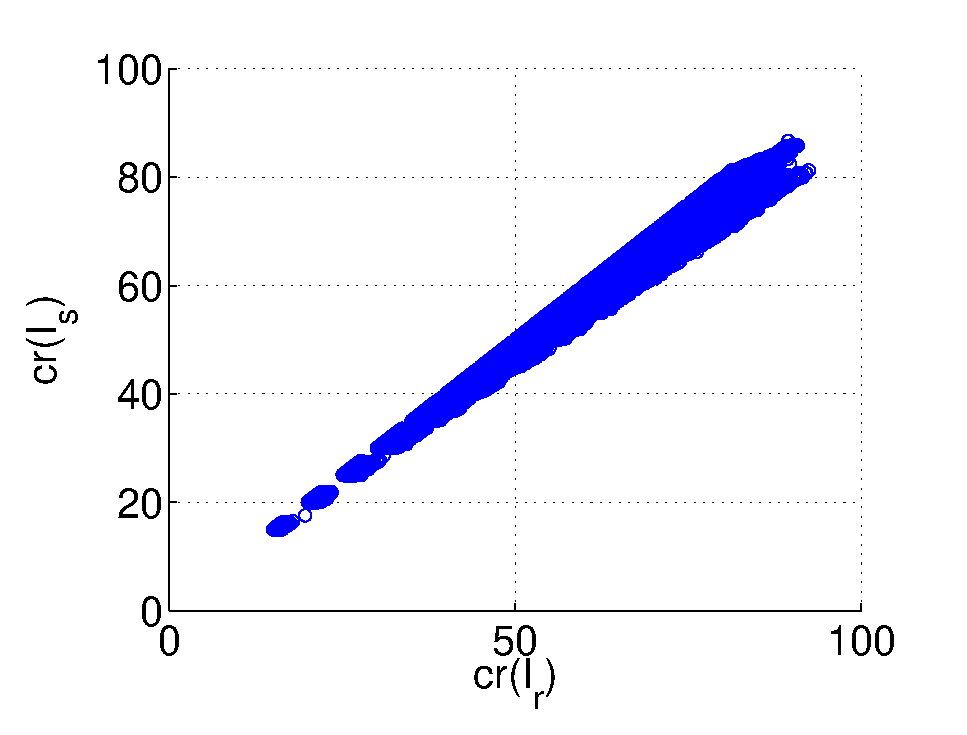
\includegraphics[width=0.45\linewidth]{img/jxrData.eps}
	
	\vspace{3mm}
	\begin{tabular}{c|c|c|c||c|c|c}
		& \multicolumn{3}{c||}{single: $1-\frac{cr(I_u, I_s)}{cr_t}$ } & \multicolumn{3}{c}{recomp.: $ 1-\frac{cr(I_u, I_r)}{cr_t}$} \\
		\hline
		\textbf{\%} & \emph{jpg} & \emph{j2k} & \emph{jxr} & \emph{jpg} & \emph{j2k} & \emph{jxr} \\
		\hline
		$ \mu $ & -3.21 & -3.48	&  -4.33 &  -6.80&   -7.04 &   -9.49 \\
		$ \sigma$ &2.74 &2.51 &  2.87 & 4.83  & 4.23  & 4.34 \\
	\end{tabular}
	
	
	\vspace{2mm}
	
	\end{small}
	
	\caption{Scatter plots of measured compression ratios $cr(I_u, I_s)$ over $cr(I_u, I_r)$ for methods \emph{jpg} (left) and \emph{jxr} (right). The graphs indicate that the $s(I_s^{(k)}) \geq s(I_r^{(k)})$ condition from equ. (\ref{equ:recomp}) is satisfied. While this is indeed true for \emph{j2k} and \emph{jxr}, we observe a violation in 0.13\% of the cases for \emph{jpg} at $cr_t \geq 70$, because JPEG is already working at it's boundaries at such high compression ratios. The table below reveals, that in average the aimed $cr_t$ is met with 3.67\% accuracy for single-compressed images $I_s$, while the re-compressed ones $I_r$ only reach 7.8\%. This is due to the limited universe of quality parameters $q, q_p$.}
	
	
	\label{fig:dataDistribution}
\end{figure}

\section{Evaluation}
\label{section:eval}
 We investigate the behavior of iris segmentation employing a segmentation error rate (section \ref{section:ser}). Besides that, we assess the image quality with fully-referenced metrics (section \ref{section:fulRef}). The individual results are then compared in \ref{section:comparison}.


\subsection{Full-referenced quality metrics}
\label{section:fulRef}
Evaluating the quality of the compressed images in respect to the original an assortment of full-reference metrics was chosen. The choice was made according to different aspects of human perception starting from mathematically defined to low-level features based and finally to high-level features based. The following were included: 
 
\begin{itemize}
 \item PSNR: Peak signal-to-noise ratio
 \item MSSIM\cite{Wangsa}: Multi-scale structural similarity index  is an extension of the SSIM metric. After the extraction of luminance, structure and contrast components from the image at scale 1, the algorithm iteratively applies a low pass filter and a downsamples the
 filtered image by a factor of 2. The overall result is the combination of measurements at different scales.
 \item NQM\cite{Dameraa}: Noise Quality Measure, a low-level HVS features based metric. The contrast pyramid of Peli’s work was used to model the variation in contrast, sensitivity with distance, dimensions and spatial frequency of the stimuli, and with the variation of their local luminance mean.
 \item RFSIM\cite{Zhanga}: Riesz-transform feature based similarity metric approximates HVS by perceiving an image mainly according to its low-level features. Uses the 1st-order and 2nd-order Riesz transform coefficients. The similarity index is measured by comparing the two feature maps at key locations marked by the feature mask. The mask is generated by a Canny operator.
 \item VSNR\cite{Chandlera}: Visual Signal-to-Noise Ratio, a wavelet based
 metric. The metric is designed to evaluate both low-level and
 mid-level HVS features. VSNR works in two stages: the first computes the contrast detection thresholds, while the second estimates visual fidelity by measuring the perceived contrast and the extent to which
 the distortions disrupt global precedence
 
\end{itemize}

Applying these quality metrics \emph{jpg}, \emph{j2k} and \emph{jxr} resulted in the following observations in fig. 3 \& 4. It is observed that:
\begin{enumerate}
	\item For \emph{jpg} and $cr_t>15 $ single compressed images were of higher quality compared to re-compressed and
		 at $cr_t$=15 the single compressed images were of the lowest quality as shown in fig. 3 for MSSIM.
		 The quality of the re-compressed images followed the trend that the higher the $q_p$ the better the quality of the image. Previous observation of metrics for jpg was unanimous for all metrics.
	
	\item For \emph{jk2} in all compression ratios and all metrics, the quality of the re-compressed images followed the trend that the higher the $q_p$ the better the quality of the image. Single compressed images were of the highest quality compared to re-compressed data, which was valid for all metrics and compression ratios as shown for MSSIM in fig. 3 	 
			  
	
		\item For \emph{jxr} and $15\leq{cr_t}\leq{40}$ single compressed images were of the lowest quality compared to re-compressed data for MSSIM and VSNR. The latter followed the trend of the higher the $q_p$ the better the quality of the image fig.4		 
        For $45\leq{cr_t}\leq{75}$ images of single compression became of the highest quality and  re-compressed data continued the same trend for MSSIM and VSNR metrics.
        NQM showed the same behaviour, but ${cr_t}$=50 was observed to be the changing point in this case. RFSIM showed a different trend from the previous; single compressed data were always of the best quality compared to re-compressed data which followed in terms of quality measurement. 
   
   
   
\end{enumerate}

\begin{figure}[!h]
	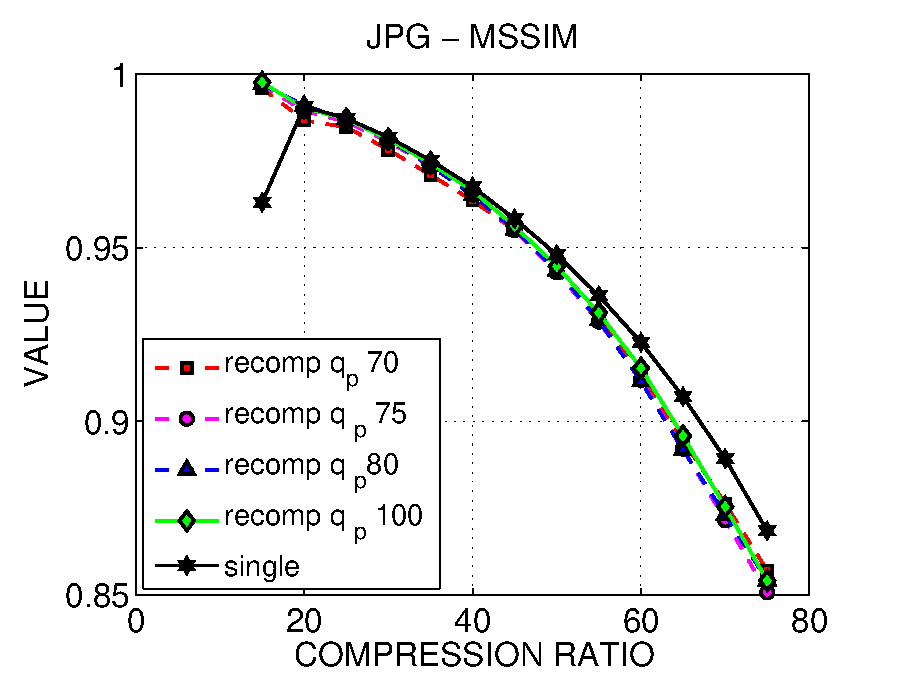
\includegraphics[width=0.49\linewidth]{img/new/mssim_jpg.eps}
	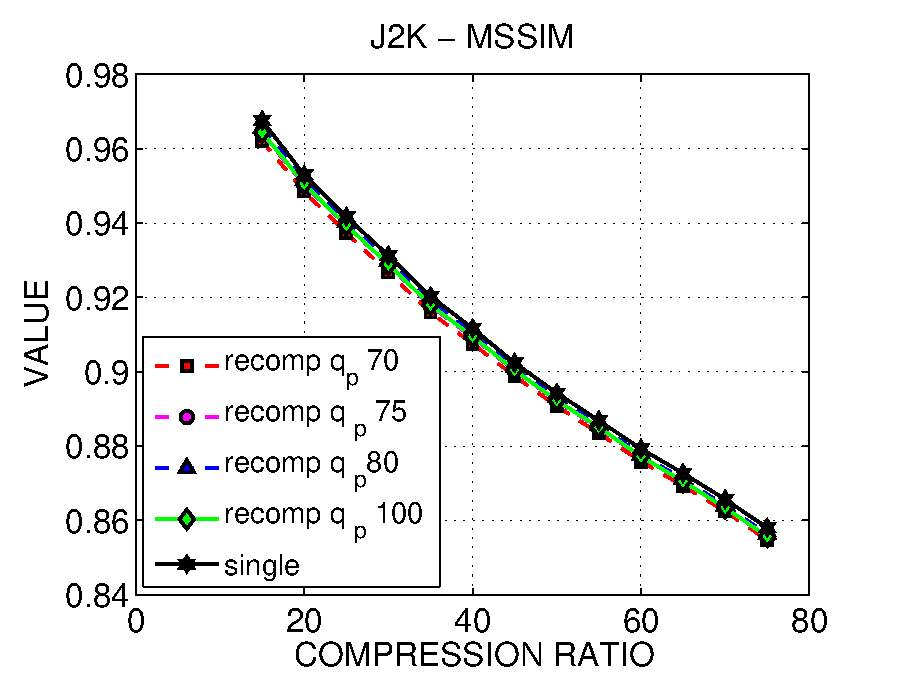
\includegraphics[width=0.49\linewidth]{img/new/j2k_mssim.eps}	
	
	\caption{Left: MSSIM of \emph{jpg} single- and recompressed data. Right: MSSIM of \emph{jp2} single- and recompressed data}
	\label{fig:mssim}
\end{figure}


\begin{figure}[!h]
	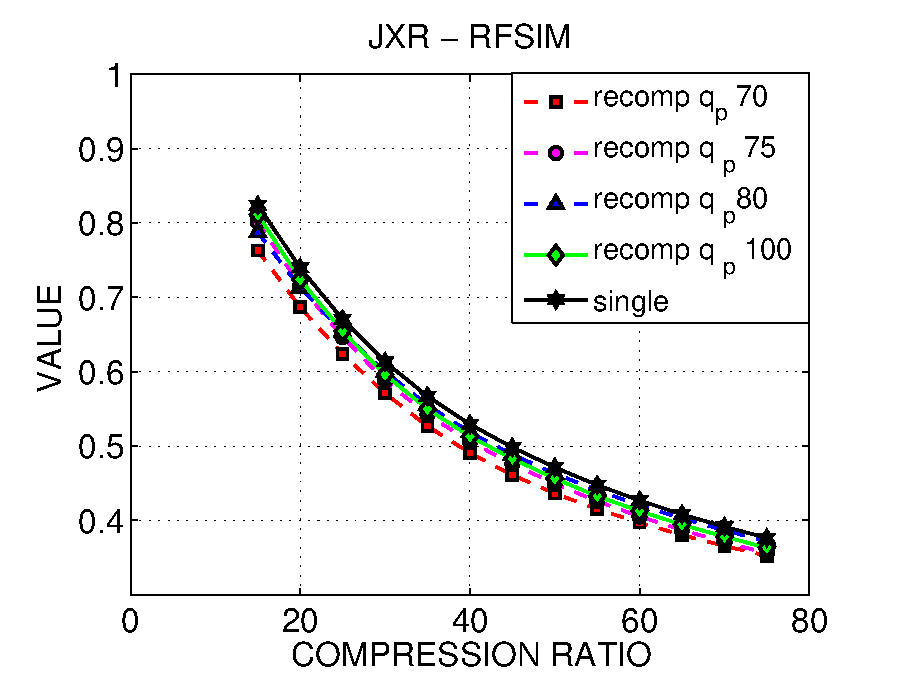
\includegraphics[width=0.49\linewidth]{img/new/rt_jxr.eps} %jxr_psnr.eps
	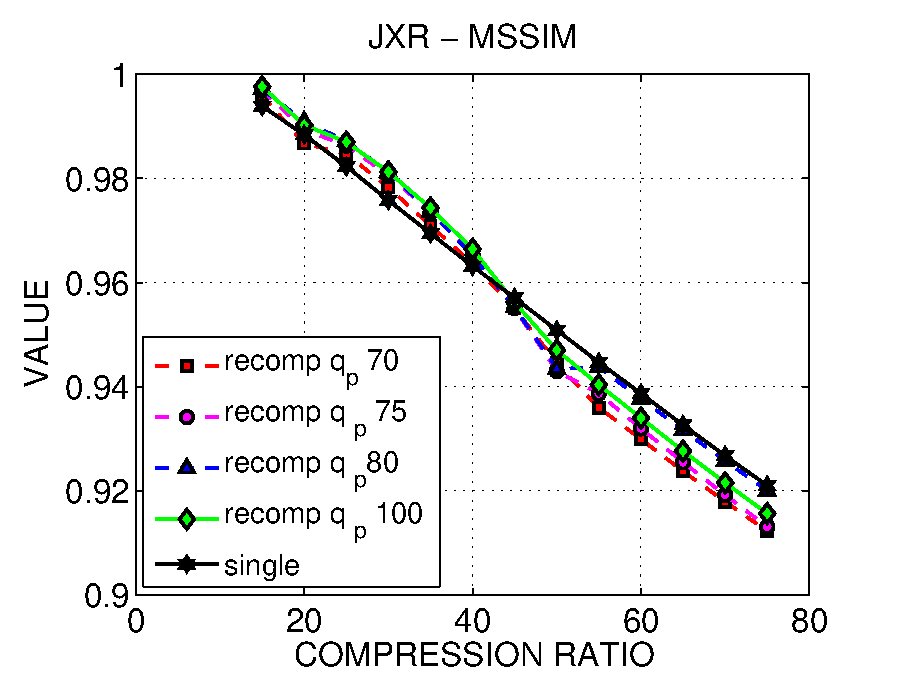
\includegraphics[width=0.49\linewidth]{img/new/jxr_mssim.eps}	
	
	\caption{Left: RFSIM of \emph{jxr} single- and recompressed data. Right: MSSIM of \emph{jxr} single- and recompressed data}	
	\label{fig:psnr}
\end{figure}



\subsection{Segmentation error rates}
\label{section:ser}
In iris recognition, the segmentation of an iris image is considered as one of the most critical parts \cite{BDaugman08a, severeCompression}. %Marked for deletion
We investigate the differences of single- and recompression as well as the aspects of which reference to use. We distinguish between using an absolute reference, e.g. a ground truth, and a relative one, e.g. the segmentation of the uncompressed images $I_u$, when computing the error rate.

\begin{figure}
\begin{center}

  
\includegraphics[width=0.3\linewidth]{img/segMasks/gt.png}
  
\includegraphics[width=0.3\linewidth]{img/segMasks/jpg_caht_q100_cr5.png}
  
\includegraphics[width=0.3\linewidth]{img/segMasks/jpg_wahet_q100_cr5.png}
  \end{center}
  
  \label{fig:segMasks}
  \caption{Segmentation masks of the expert ground truth \cite{Hofbauer14b}, relative groundtruth $seg(I_u^{(k)})$ and an actual segmentation result $seg(I_r^{(k)})$ (f.l.t.r)}
\end{figure}

%TODO discuss, why the eye lashes are notmasked in the algos


The segmentation accuracy is rated by the mean segmentation error rate, which corresponds to the suggested E1 error rate in the Noisy Iris Challenge Evaluation - Part I (NICE.I). We define the segmentation error rate $ser$ as
\begin{equation}
ser(R,S) = \overline{R \oplus S} \in [0,1]\quad with \quad R,S \in \{0,1\}^{w \times h},
\end{equation} where $R$ is the binarized reference segmentation and $S$ the binarized segmentation result of the same image $I$. The mean value of the pixel-wise exclusive-or is the percentage of pixels different in the segmented image $S$ in respect to the reference $R$. Due to multiple images in a data base, the mean segmentation error $mser$ is computed from $K$ images. We compute the absolute mean segmentation error $mser_{abs}$ in respect to the ground truth $SGT$ and the relative mean segmentation error $mser_{rel}$ in respect to the segmentation of the uncompressed images $I_u$ for single- and recompressed images $I_c \in {I_s, I_r}$. By denoting the segmentation result of an image $I$ as $seg(I) \in \{0,1\}^{w \times h}$ we have
\begin{eqnarray}
mser_{abs} = \frac{1}{K}\sum_{k=1}^{K}ser(SGT^{(k)},seg(I_c^{(k)})) \label{equ:mserabs} \\
mser_{rel} = \frac{1}{K}\sum_{k=1}^{K}ser(seg(I_u^{(k)}),seg(I_c^{(k)})) \label{equ:mserrel}
\end{eqnarray}

The absolute segmentation error rate is considered to be optimal because of the available ground truth. However, for most data bases no such ground truth is available. Therefore we evaluate if the same conclusions as from the $mser_{abs}$ can be drawn from the $mser_{rel}$. The benefit of such a relation (if it exists) is that the $mser_{rel}$ can be computed for any arbitrary data set. 

\begin{figure}
	\begin{center}
		
	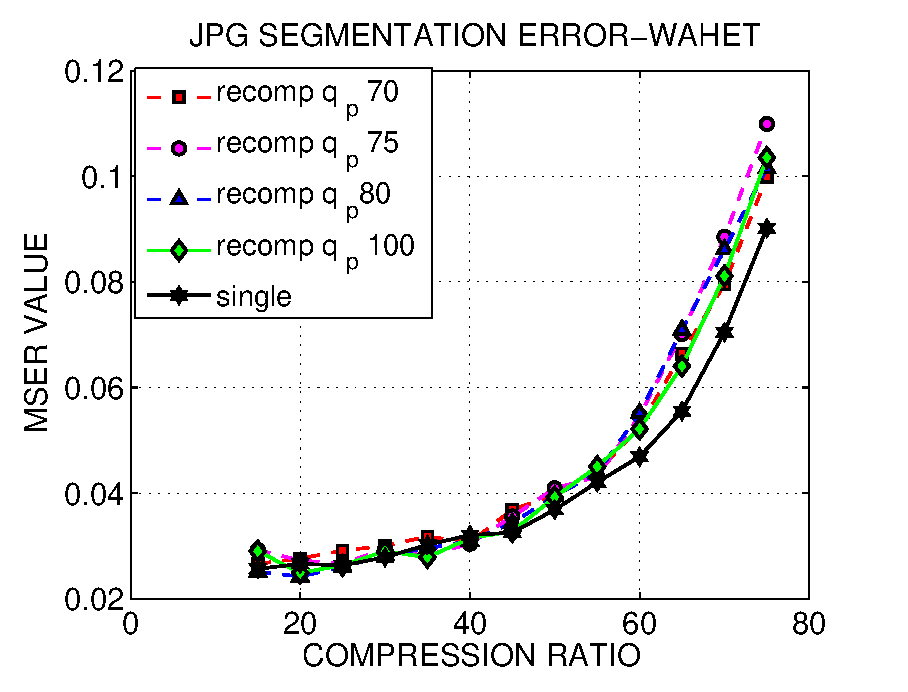
\includegraphics[width=0.49\linewidth]{img/new/jpg_wahet.eps}
	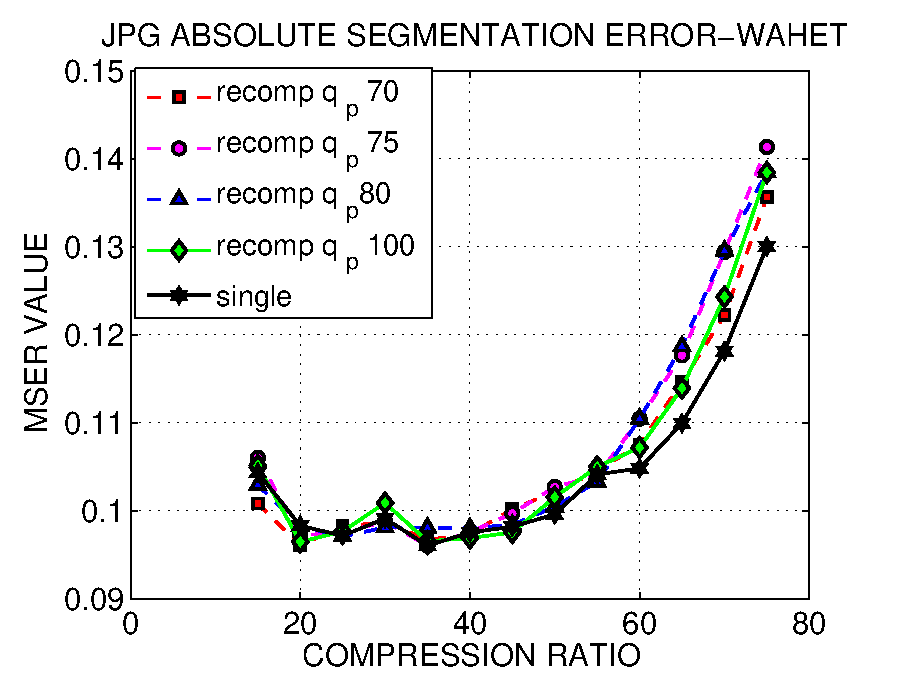
\includegraphics[width=0.49\linewidth]{img/new/jpg_abs_wahet.eps}
	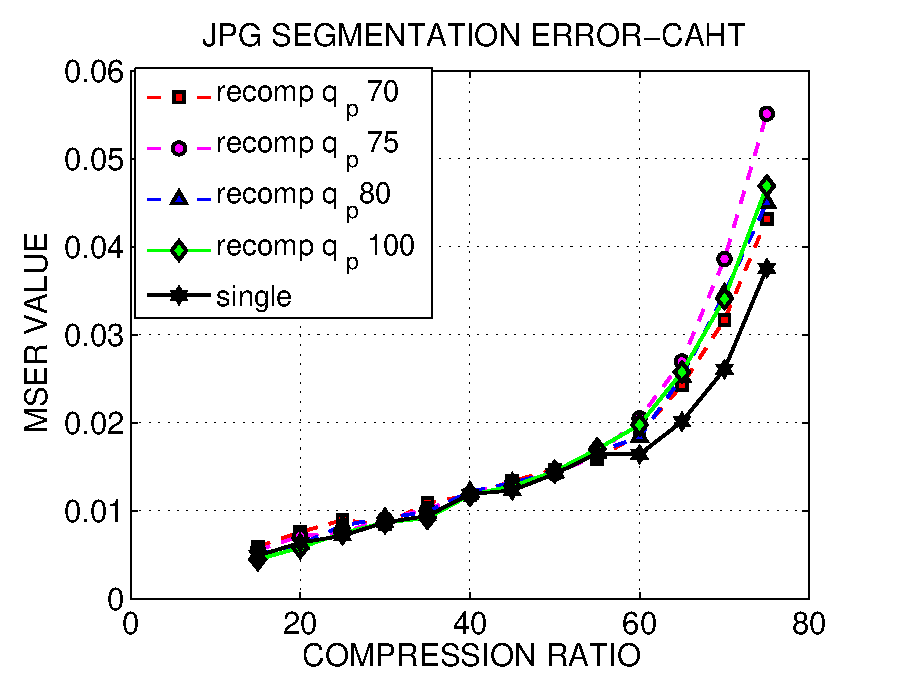
\includegraphics[width=0.49\linewidth]{img/new/jpg_caht.eps}
	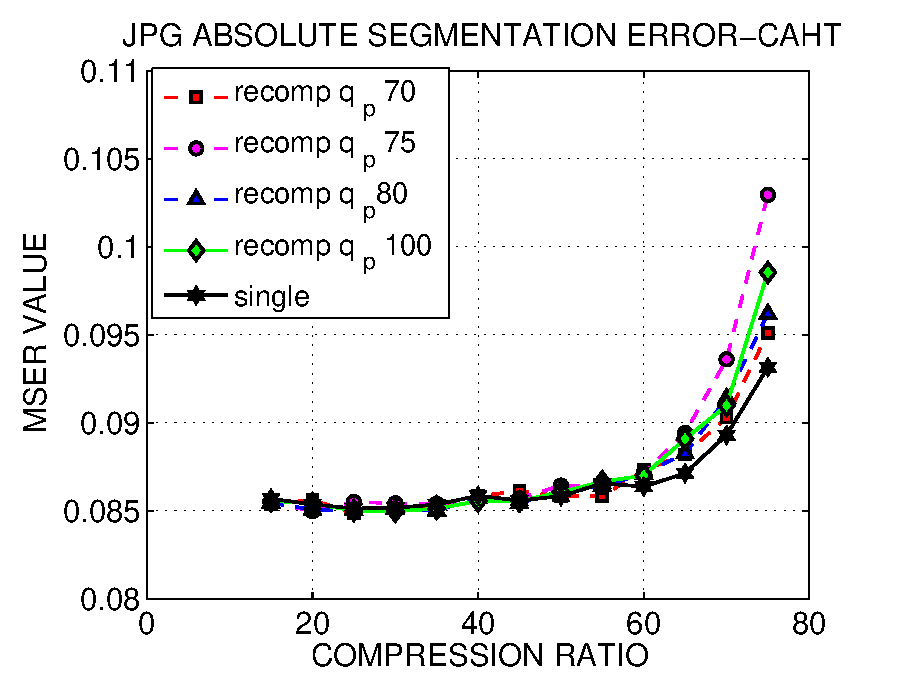
\includegraphics[width=0.49\linewidth]{img/new/jpg_abs_caht.eps}
	
\end{center}
	\caption{Relative and absolute segmentation error $mser_{rel}$ (left) and $mser_{abs}$ (right) with WAHET (top) and CAHT (bottom) segmentation on $jpg$-compressed data. Note that the $mser_{abs}$ is generally higher than $mser_{rel}$, because the tested algorithms ignore eyelids, yet they are considered in the expert ground truth \cite{severeCompression}.}
	\label{fig:segResultsJPG}
	
\end{figure}

\begin{figure}
	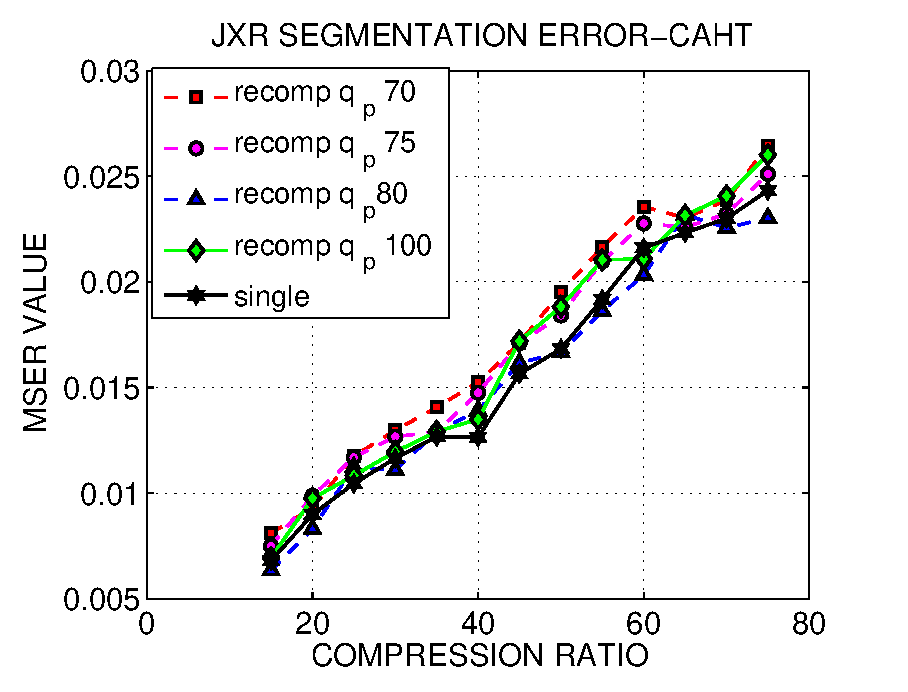
\includegraphics[width=0.49\linewidth]{img/new/jxr_caht.eps}
	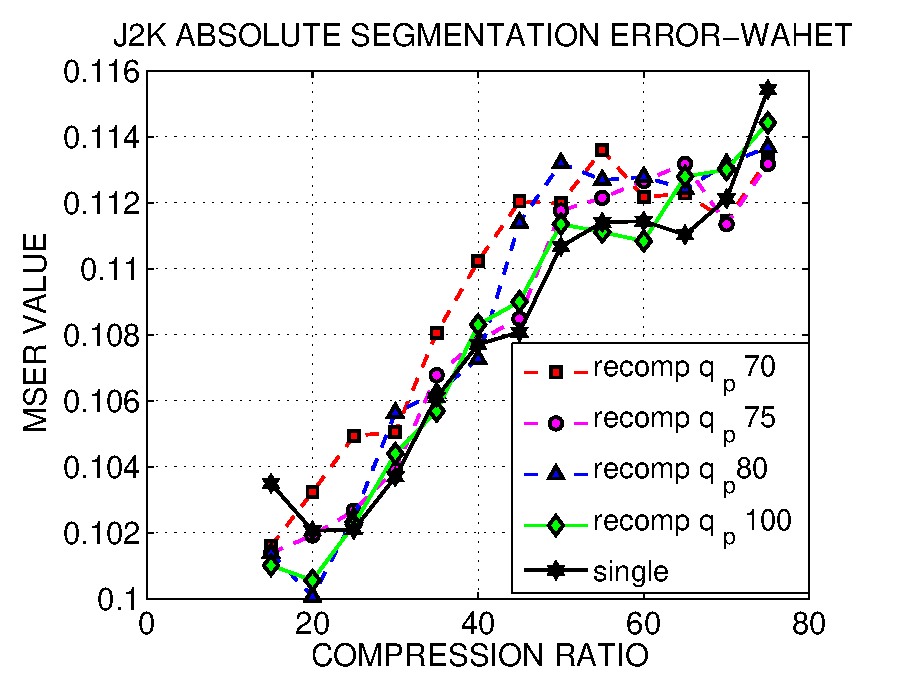
\includegraphics[width=0.49\linewidth]{img/new/j2k_abs_wahet.eps}	
	\caption{Relative CAHT segmentation error rate $mser_{rel}$ for \emph{jxr}-compressed data (left) and absolute WAHET segmentation error rate $mser_{abs}$ for \emph{jp2}-compressed data (right)}
	\label{fig:segResultsOther}
\end{figure}


The data set described in section \ref{section:exSetup} is used to test the two iris segmentation algorithms, Contrast-adjusted Hough Transform (CAHT) and Weighted Adaptive Hough and Ellipsopolar Transform (WAHET), from the USIT Framework v1.0.3\footnote{as available at \url{http://wavelab.at/sources/} \cite{Rathgeb12e}}. From the results we observe the following:

\begin{enumerate}
	\item Results for intra-recompression experiments, namely \emph{jpg} on \emph{jpg} pre-compressed data, in figure \ref{fig:segResultsJPG} indicate:  
	
	
	\begin{enumerate}
		\item For small and medium compression ratios ($ cr_t \leq 50 $) no significant difference in segmentation errors of single- and recompressed data is observeable. This implies that for these compression ratios it has no impact whether pre-compressed or uncompressed data is used in experiments. \label{noDiff}
		\item For large compression ratios ($cr_t > 50$), segmentation errors tend to be lower for single-compressed data compared to recompressed data. Thus using pre-compressed or uncompressed data in experiments matters. \label{yesDiff} 
		 
		 \item $mser_{rel}$ and $mser_{abs}$ generally show the similar trends for medium and large compression ratios, i.e. there is a strong correlation of  $mser_{rel}$ and $mser_{abs}$ for $cr_t > 30$. This means, the relative error $mser_{rel}$ suffices to rate performance on iris segmentation here, implying no expert-generated ground truth is needed. \label{gtNoHigh}
		 
		 \item However, WAHET segmentation errors reveal that in some cases there can be a difference between $mser_{rel}$ and $mser_{abs}$ for $cr_t \leq 30$. Figure \ref{fig:segResultsJPG} shows here a different behaviour between absolute error $mser_{abs}$ (top-right) and relative error $mser_{rel}$ (top-left). Hence, for low compression ratios a ground truth is required. \label{gtForLow}
		 
		 \item In recompression, one might expect a linear relation between used pre-compression quality $q_p$ and ranking of the error rates. Interestingly, when looking at figure \ref{fig:segResultsJPG} at high compression ratios, the poorest performance corresponds to $q_p=75$, while the best is related to $q_p=70$. In contradiction, $q_p=100$ performs significantly better than $q_p=80$ in most settings.   \label{qpConfusion}
	\end{enumerate}
 
 
 \item There are no clear trends for inter-recompression experiments, namely \emph{jxr} or \emph{j2k} on \emph{jpg} pre-compressed data. Even so, some interesting observations are made, which are illustrated figure \ref{fig:segResultsOther}:
 
 \begin{enumerate}
 	 	\item Data generated in a single compression step generally tends to result in smaller error rates compared to those computed from recompressed data. Interestingly, for extreme values, namely very small and very large compression ratios, single-compression performs often poorer. \label{singleAmongBest}
 	 	
 	 	\item For all experiments carried out with \emph{jxr} and \emph{jp2}, the error rate stagnates in some way for medium compression ratios, i.e. $45 \leq cr_t \leq 70$. Exemplarily this can be seen in the $mser_{abs}$ for \emph{jp2}-method (figure \ref{fig:segResultsOther} left). The characteristics of a curve's stagnancy vary depending on the pre-compression quality $q_p$. Since stagnancy can be seen in single- as well as recompressed data, we conclude the effect is generally related to the used methods \emph{jxr} and \emph{jp2}. However, the characteristics of the stagnancy seem be controlled by the pre-compression quality $q_p$ in a way that the lower the pre-compression quality is, the clearer the curve stagnates. \label{cureFlattening}
\end{enumerate}  
  \end{enumerate}
 
\paragraph{In (jpg) intra-recompression,} recompression effects have a strong impact on experimental results for large compression ratios, i.e. $cr_t > 50$ (\ref{noDiff}, \ref{yesDiff}). Researchers are often forced to use precompressed data sets for the sake of ground truth availability. Results for compression ratios of $cr_t > 50$ can therefore not be considered entirely reliable (\ref{yesDiff}). However, recompression effects have negative influence on segmentation error rates, hence by using uncompressed data for the same experiments, better results may be achieved. If this behaviour is related to intra-recompression in general or for \emph{jpg}-recompression only, is topic to further research.

From \ref{gtNoHigh} we know that for large compression ratios, i.e. $cr_t > 50$, there is no difference in the progress of $mser_{rel}$ and $mser_{abs}$. Since this is (from \ref{yesDiff}) exactly the range, where using single- or recompressed data does have an impact, we propose - based on observations \ref{gtForLow} and \ref{gtNoHigh} - to bench-mark compression algorithms in respect to iris segmentation by using 
\begin{itemize}
	
	\item \vspace{-1.5mm} uncompressed data sets rated with relative measures, such as the $mser_{rel}$, for severe compression, i.e. $cr_t > 50$ and
	\item \vspace{-2mm}pre-compressed data sets\footnote{If absolutely necessary because of ground-truth availability, of course uncompressed data is preferred} with absolute measures, such as $mser_{abs}$, for medium and light compression, i.e. $cr_t \leq 50$.
\end{itemize}

If this applies to intra-compression with other methods as well needs further investigation.

\paragraph{In inter-recompression} we cannot observe such behaviour. However, there are trends observeable (\ref{singleAmongBest}, \ref{cureFlattening}), which need further investigation. 


\section{Comparison}
\label{section:comparison}
Besides evaluating the segmentation error rate and the general purpose quality measures independently, their correlation is analysed. Furthermore, we explicitly investigate the correlation between $mser_{rel}$ and $mser_{abs}$ to back up the observations in section \ref{section:ser}.
For this purpose, we used the Spearman's rank correlation coefficient (SRCC).

In general, all five used general purpose quality metrics show a high linear relationship with a minimum SRCC of $0.852$ to each other. Furthermore, all of these metrics are highly correlating with the segmentation error rate and there are only minor differences between the segmentation algorithms (WAHET and CAHT) and the relative and absolute segmentation error rates. Table \ref{tab:corrJPG} shows the correlation results for the intra-compression (\emph{jpg}) and the CAHT segmentation algorithm. It can be observed that the $mser_{rel}$ shows overall a higher linear relationship to the quality metrics than the $mser_{abs}$. The reason for this can be seen in Figure \ref{fig:segResultsJPG} (bottom) where the $mser_{rel}$ has a higher slope for small and medium CRs where the $mser_{rel}$ is more flat in this region and is in general more noisy as well.
Furthermore, it can be seen that for the MSSIM metric ($mser_{rel}$) in case of single compression the SRCC is smaller compared to the other metrics, which is due to the outlier of the MSSIM at $cr_t = 15$ in Figure \ref{fig:mssim}. However, except of this outlier and when looking at the graphs as well, the MSSIM represents best the segmentation error rates in case of the intra-compression, because the single compressed curve gets away from the bundle of the recompressed curves for high compression ratios (compare figure \ref{fig:mssim} left and \ref{fig:segResultsJPG}).
On the other hand, on jp2 compressed data (figure \ref{fig:mssim} right) MSSIM shows absolutely no sign of the stagnancy, although there is clear stagnancy in figure \ref{fig:segResultsOther} (left). Hence, MSSIM (among others) cannot be used to predict behaviour of iris segmentation. This could also mean that the segmentation not only depends on the quality of an image, or at least not in a linear relationship. 

\begin{table}\footnotesize\centering
\begin{tabular}{ | l || l | l | l | l | l | }
    \hline
    \multicolumn{6}{|c|}{SRCC between the quality metrics and the relative MSER} \\
    \hline
    & \emph{single} & \emph{rec.70} & \emph{rec.75} & \emph{rec.80} & \emph{rec.100} \\ \hline
    \emph{PSNR} & -0.995 \cellcolor[rgb]{0,0.5,0} & -0.995 \cellcolor[rgb]{0,0.5,0} & -1.0 \cellcolor[rgb]{0,0.5,0} & -1.0 \cellcolor[rgb]{0,0.5,0} & -1.0 \cellcolor[rgb]{0,0.5,0} \\ \hline
    \emph{MSSIM} & -0.912 \cellcolor[rgb]{0,0.5,0} & -0.995 \cellcolor[rgb]{0,0.5,0} & -1.0 \cellcolor[rgb]{0,0.5,0} & -1.0 \cellcolor[rgb]{0,0.5,0} & -1.0 \cellcolor[rgb]{0,0.5,0} \\ \hline
    \emph{NQM} & -0.995 \cellcolor[rgb]{0,0.5,0} & -0.995 \cellcolor[rgb]{0,0.5,0} & -1.0 \cellcolor[rgb]{0,0.5,0} & -1.0 \cellcolor[rgb]{0,0.5,0} & -1.0 \cellcolor[rgb]{0,0.5,0} \\ \hline
    \emph{VSNR} & -0.995 \cellcolor[rgb]{0,0.5,0} & -0.995 \cellcolor[rgb]{0,0.5,0} & -1.0 \cellcolor[rgb]{0,0.5,0} & -1.0 \cellcolor[rgb]{0,0.5,0} & -1.0 \cellcolor[rgb]{0,0.5,0} \\ \hline
    \emph{RFSI} & -0.995 \cellcolor[rgb]{0,0.5,0} & -0.995 \cellcolor[rgb]{0,0.5,0} & -1.0 \cellcolor[rgb]{0,0.5,0} & -1.0 \cellcolor[rgb]{0,0.5,0} & -0.995 \cellcolor[rgb]{0,0.5,0} \\ \hline
    \hline
    
    \multicolumn{6}{|c|}{SRCC between the quality metrics and the absolute MSER} \\
    \hline
    & \emph{single} & \emph{rec.70} & \emph{rec.75} & \emph{rec.80} & \emph{rec.100} \\ \hline
    \emph{PSNR} & -0.857 \cellcolor[rgb]{0,0.5,0} & -0.863 \cellcolor[rgb]{0,0.5,0} & -0.929 \cellcolor[rgb]{0,0.5,0} & -0.868 \cellcolor[rgb]{0,0.5,0} & -0.841 \cellcolor[rgb]{0,0.5,0} \\ \hline
    \emph{MSSIM} & -0.923 \cellcolor[rgb]{0,0.5,0} & -0.863 \cellcolor[rgb]{0,0.5,0} & -0.929 \cellcolor[rgb]{0,0.5,0} & -0.868 \cellcolor[rgb]{0,0.5,0} & -0.841 \cellcolor[rgb]{0,0.5,0} \\ \hline
    \emph{NQM} & -0.857 \cellcolor[rgb]{0,0.5,0} & -0.863 \cellcolor[rgb]{0,0.5,0} & -0.929 \cellcolor[rgb]{0,0.5,0} & -0.868 \cellcolor[rgb]{0,0.5,0} & -0.841 \cellcolor[rgb]{0,0.5,0} \\ \hline
    \emph{VSNR} & -0.857 \cellcolor[rgb]{0,0.5,0} & -0.863 \cellcolor[rgb]{0,0.5,0} & -0.929 \cellcolor[rgb]{0,0.5,0} & -0.868 \cellcolor[rgb]{0,0.5,0} & -0.841 \cellcolor[rgb]{0,0.5,0} \\ \hline
    \emph{RFSI} & -0.857 \cellcolor[rgb]{0,0.5,0} & -0.863 \cellcolor[rgb]{0,0.5,0} & -0.929 \cellcolor[rgb]{0,0.5,0} & -0.868 \cellcolor[rgb]{0,0.5,0} & -0.846 \cellcolor[rgb]{0,0.5,0} \\ \hline

\end{tabular}
\caption{Spearman Rank Correlation Coefficient between the quality metrics and the $mser_{rel}$ (above) as well as the $mser_{abs}$ (below) for intra-compression (\emph{jpg}) and the CAHT segmentation algorithm.}
\label{tab:corrJPG}
\end{table}

%\textbf{Note by TB}: Although MSSIM (figure \ref{fig:mssim}) shows a strong correlation to jpg related segmentation error rates, because also the single compressed curve gets away from the bundle of the other curves, MSSIM on jp2 compressed data (figure \ref{fig:mssim})  shows absolutely no sign of the stagnancy, although there is clear stagnancy in figure \ref{fig:segResultsOther} (left). Hence, MSSIM (among others) cannot be used to predict behaviour of iris segmentation. This could also mean that the segmentation NOT ONLY depends on the quality of an image, or at least not in a linear relationship.

%This becomes even more obvious when comparing figure \ref{fig:psnr} with \ref{fig:segResultsOther}, although for pre-compression 85 at least a step from 50-55 can be seen. Pls make similar observations here...

The SRCC between the relative and absolute segmentation error rates confirms that both metrics the same trend as it can be seen in Table \ref{tab:corrMSER}. In case of the WAHET segmentation \emph{jp2} outperforms the other two compression methods. The smaller SRCC values for \emph{jpg} is mainly due to the $mser_{abs}$ at smaller compression ratios where the segmentation error rate is higher for $cr_t = 15$ than for $cr_t = 20$. Also the small ripple at $cr_t = 30$ has an impact on the correlation here.
The reason for the intermediate SRCC results in case of jxr are mainly due to noise, which can be seen in Figure \ref{fig:segResultsOther}.


\begin{table}\footnotesize\centering
\begin{tabular}{ | l || l | l | l | l | l | }
    \hline
    \multicolumn{6}{|c|}{WAHET Segmentation} \\
    \hline
    & \emph{single} & \emph{rec.70} & \emph{rec.75} & \emph{rec.80} & \emph{rec.100} \\ \hline
    \emph{jpg} & 0.703 \cellcolor[rgb]{0,0.8,0} & 0.835 \cellcolor[rgb]{0,0.5,0} & 0.890 \cellcolor[rgb]{0,0.5,0} & 0.786 \cellcolor[rgb]{0,0.8,0} & 0.863 \cellcolor[rgb]{0,0.5,0} \\ \hline
    \emph{j2k} & 0.978 \cellcolor[rgb]{0,0.5,0} & 0.962 \cellcolor[rgb]{0,0.5,0} & 0.978 \cellcolor[rgb]{0,0.5,0} & 0.923 \cellcolor[rgb]{0,0.5,0} & 0.978 \cellcolor[rgb]{0,0.5,0} \\ \hline
    \emph{jxr} & 0.742 \cellcolor[rgb]{0,0.8,0} & 0.956 \cellcolor[rgb]{0,0.5,0} & 0.423 \cellcolor{orange} & 0.544 \cellcolor[rgb]{0,0.8,0} & 0.412 \cellcolor{orange} \\ \hline
    \hline
    
    \multicolumn{6}{|c|}{CAHT Segmentation} \\
    \hline
    & \emph{single} & \emph{rec.70} & \emph{rec.75} & \emph{rec.80} & \emph{rec.100} \\ \hline
    \emph{jpg} & \cellcolor[rgb]{0,0.5,0} 0.863 & \cellcolor[rgb]{0,0.5,0} 0.802 & \cellcolor[rgb]{0,0.5,0} 0.928 & \cellcolor[rgb]{0,0.5,0} 0.868 & \cellcolor[rgb]{0,0.5,0} 0.841 \\ \hline
    \emph{j2k} & \cellcolor[rgb]{0,0.5,0} 0.984 & \cellcolor[rgb]{0,0.5,0} 1.0 & \cellcolor[rgb]{0,0.5,0} 0.995 & \cellcolor[rgb]{0,0.5,0} 1.0 & \cellcolor[rgb]{0,0.5,0} 1.0 \\ \hline
    \emph{jxr} & \cellcolor[rgb]{0,0.5,0} 0.978 & \cellcolor[rgb]{0,0.5,0} 0.973 & \cellcolor[rgb]{0,0.5,0} 0.967 & \cellcolor[rgb]{0,0.5,0} 0.918 & \cellcolor[rgb]{0,0.5,0} 0.978 \\ \hline

\end{tabular}
\caption{SRCC between $mser_{rel}$ and $mser_{abs}$ for all three methods and both WAHET segmentation (above) and CAHT segmentation (below).}
\label{tab:corrMSER}
\end{table}



\section{Conclusion}
\label{section:conclusion}
Iris biometrics compression performance is usually rated in experimental setups. Often researchers use JPEG pre-compressed data for these experiments, quite frequently because of ground-truth availability. We investigated whether the outcome of such experiments can be considered reliable by comparing segmentation error and quality metrics of single-compressed and re-compressed data.  In the segmentation error rate, no tendency is observeable when comparing single-compression and inter-recompressed data. However, using intra-recompressed data, i.e. compressing JPEG pre-compressed data with JPEG again, a different behaviour is observed for high compression ratios compared to single-compressed data sets. Thus results of studies using JPEG compression on JPEG pre-compressed data cannot be considered entirely reliable. We showed for small compression ratios, a ground truth is indeed necessary for accurate segmentation error rating. Furthermore, we propose a method to overcome such problems in section \ref{section:ser}. Interestingly, there seems to be no strictly linear relation between image quality and segmentation error rate. Quality metrics tend to omit detailed behaviour of the segmentation error in respect to compression ratios. Nevertheless, quality metrics and segmentation error follow the same trends and metrics such as the MSSIM can therefore be used to estimate an iris segmentation algorithms behavior. 

So far only the impact on iris segmentation has been considered. Recompression artifacts potentially influence other parts of an iris recognition system, e.g. iris code generation. This is topic to further research.           


{\small
\bibliographystyle{ieee}
\bibliography{egbib}
}

\end{document}
